\section{主成分分析}
\label{sec:chapter12}

\subsection{数据降维}

我们的数据特征常常包含众多维度，但它们中的有些维度其实没有存在的必要。最极端的情况就是某一维度是其他若干维度的线性组合，那么这一维度就完全可以丢掉；但现实不会这么精准，如果某一维度是其他若干维度的线性组合加上微小的扰动，我们其实也可以将其丢掉。这就是数据降维。

\begin{figure}[H]
    \centering
    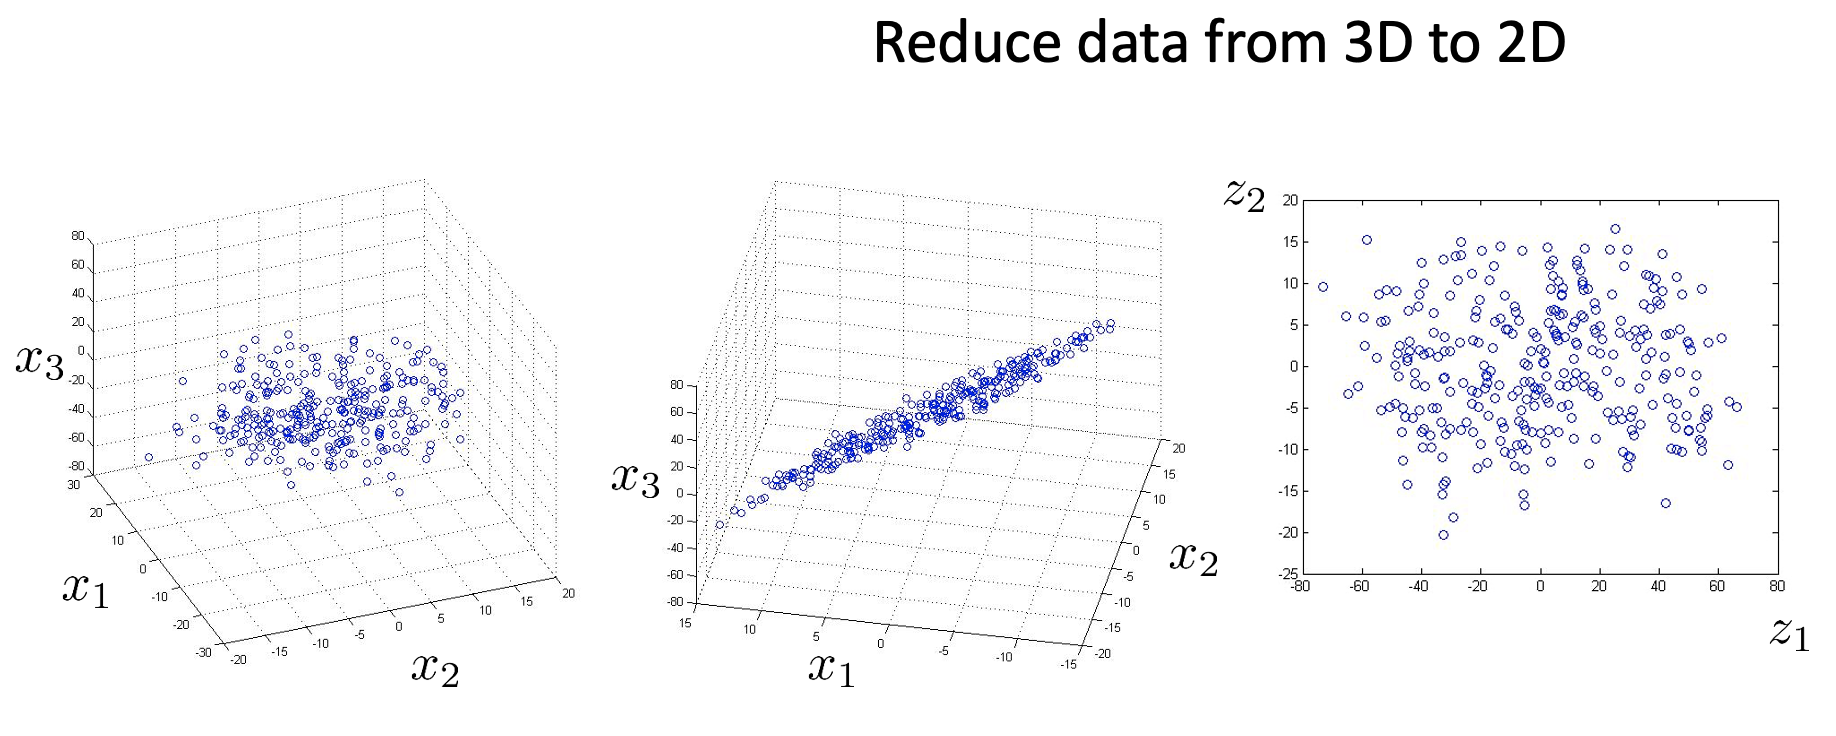
\includegraphics[width=\linewidth]{figs/Chap_12_data_compression.png}
\end{figure}

数据降维有众多算法可以完成，主成分分析即是其中之一。


\subsection{主成分分析}

主成分分析（Principal Component Analysis）的基本思想是：假设原始数据的特征有 $n$ 维，我们想将其缩减到 $k$ 维，那么我们只需要在原来的 $n$ 维空间中找到一个 $k$ 维的子空间，使得所有数据到这个子空间的距离平方和最小；此时，原数据在这个子空间上的投影就是我们新的 $k$ 维的数据。

\paragraph{数学推导}

为方便，我们首先将数据中心化，即使得数据的平均值在原点处。<u>一个获得所需要的 $k$ 维子空间的简单方式是：找到一个合适的 $n$ 维空间，直接选取前 $k$ 维作为子空间</u>。具体而言，对于一个数据点 $x=\begin{bmatrix}x_1\\x_2\\\vdots\\x_n\end{bmatrix}\in\mathbb R^n$，设我们要找的 $n$ 维空间的规范正交基为 $u_1,u_2,\ldots,u_n$，则 $x$ 在其中的新坐标为：
\[
y_j=x\cdot u_j=x_1u_{j1}+x_2u_{j2}+\cdots+x_nu_{jn}
\]
它到前 $k$ 维形成的子空间（即以 $u_1,u_2,\ldots,u_k$ 为基底的子空间）的距离之平方为：
\[
{y_{k+1}}^2+{y_{k+2}}^2+\cdots+{y_n}^2
\]
假设我们有 $m$ 个数据 $x^{(1)},x^{(2)},\ldots,x^{(m)}$，于是我们的优化目标为：
\[
\min \sum_{i=1}^m {y^{(i)}_{k+1}}^2+{y^{(i)}_{k+2}}^2+\cdots+{y^{(i)}_{n}}^2
\]
又由于在不同的基下 ${||x||}^2$ 都是一个定值，于是最小化上述距离等价于：
\[
\max \sum_{i=1}^m{y^{(i)}_1}^2+{y^{(i)}_2}^2+\cdots+{y^{(i)}_k}^2
\]
其充分条件为：
\[
\max \sum_{i=1}^m {y_r^{(i)}}^2,\quad r=1,2,\ldots,k
\]
这就是我们要解决的问题。

由于
\begin{align*}
\sum_{i=1}^m{y^{(i)}_r}^2&=\sum_{i=1}^m(x^{(i)}\cdot u_r)^2\\
&=\sum_{i=1}^m\left(u_r^Tx^{(i)}\right)\left({x^{(i)}}^Tu_r\right)\\
&=u_r^T\left(\sum_{i=1}^mx^{(i)}{x^{(i)}}^T\right) u_r
\end{align*}
这是一个正定二次型，$\sum\limits_{i=1}^mx^{(i)}{x^{(i)}}^T$ 是一个正定矩阵，可以进行奇异值分解：
\[
\sum_{i=1}^mx^{(i)}{x^{(i)}}^T=U\Sigma U^T
\]
其中，$U$ 是正交矩阵，$\Sigma$ 是对角矩阵 $\begin{bmatrix}\sigma_1&\cdots&0\\\vdots&\ddots&\vdots\\0&\cdots&\sigma_n\end{bmatrix}$，$\sigma_1,\ldots,\sigma_n$ 是奇异值，$\sigma_1>\cdots>\sigma_n$. 

令 $v_r=U^Tu_r$，由于 $U$ 正交，所以 $v_r$ 也是单位向量，代回得到：
\begin{align*}
\sum_{i=1}^m{y^{(i)}_r}^2&=u_r^TU\Sigma U^Tu_r\\
&=(U^T u_r)^T\Sigma(U^Tu_r)\\
&=v_r^T\Sigma v_r\\
&=\sigma_1v_{r1}^2+\sigma_2v_{r2}^2+\cdots+\sigma_nv_{rn}^2
\end{align*}
所以我们的优化目标变成了：
\begin{align*}
&\max\sum_{i=1}^n\sigma_iv_{ri}^2\\
&\text{s.t.}\begin{cases}\sum\limits_{i=1}^nv_{ri}^2=1\\\sigma_1>\cdots>\sigma_n\end{cases}
\end{align*}
很显然，它的解是：$v_{r1}=1,v_{r2}=\cdots=v_{rn}=0$，即 $v_r=\begin{bmatrix}1\\0\\\vdots\\0\end{bmatrix}$。又由于 $u_r=Uv_r$，<u>所以我们要找的 $n$ 维空间的各个基向量就是矩阵 $\sum\limits_{i=1}^mx^{(i)}{x^{(i)}}^T$ 的各个奇异值对应的奇异向量</u>，我们要降维到的 $k$ 维子空间的各个基向量就是前 $k$ 个奇异向量，对原来的数据进行基变换，就得到了降维后的数据。


\paragraph{步骤总结}

总结一下，主成分分析的推导过程稍显复杂，但是它的实现很简单，主要是以下步骤：

\begin{enumerate}
    \item 计算矩阵 $\sum\limits_{i=1}^mx^{(i)}{x^{(i)}}^T$；
    更简单的表达是：设矩阵 $X=\begin{bmatrix}{x^{(1)}}^T\\{x^{(2)}}^T\\\vdots\\{x^{(m)}}^T\end{bmatrix}$ 为数据集，那么计算矩阵 $X^TX$ 即可。
    \item 进行奇异值分解，得到奇异向量；
    \item 选取前 $k$ 个奇异向量作为降维后的空间的基向量，构成基变换矩阵 $C$；
    \item 对于原数据 $x$，取 $z=C^Tx$ 为其降维后的数据。
    更简单的表达是：取 $Z=XC$，则 $Z$ 是降维后的数据集。
\end{enumerate}


\paragraph{主成分数量的选择}

那么在实践中，我们到底选择多大的 $k$ 值比较好呢？对此，我们定义一个平均误差为：
\[
\frac{1}{m}\sum_{i=1}^m||x^{(i)}-x_\text{approx}^{(i)}||^2
\]
其中，$x_\text{approx}^{(i)}$ 表示数据 $x^{(i)}$ 在我们找到的 $k$ 维子空间上的投影。再定义一个总方差为：
\[
\frac{1}{m}\sum_{i=1}^m||x^{(i)}||^2
\]
则一般的，我们会选择最小的 $k$ 使得：
\[
\frac{\frac{1}{m}\sum\limits_{i=1}^m||x^{(i)}-x_\text{approx}^{(i)}||^2}{\frac{1}{m}\sum\limits_{i=1}^m||x^{(i)}||^2}\leqslant 0.01
\]
并称之为「$99\%$ 的方差得以保留」。

这个式子看起来并不好计算，但事实上，借助我们的奇异值，可以证明，对于给定的 $k$：
\[
\frac{\frac{1}{m}\sum\limits_{i=1}^m||x^{(i)}-x_\text{approx}^{(i)}||^2}{\frac{1}{m}\sum\limits_{i=1}^m||x^{(i)}||^2}=1-\frac{\sum\limits_{i=1}^k\sigma_k}{\sum\limits_{i=1}^n\sigma_i}
\]
这就好算了。


\subsection{代码实现}

\paragraph{二维压缩为一维}

二维平面上的原始数据：

\begin{figure}[H]
    \centering
    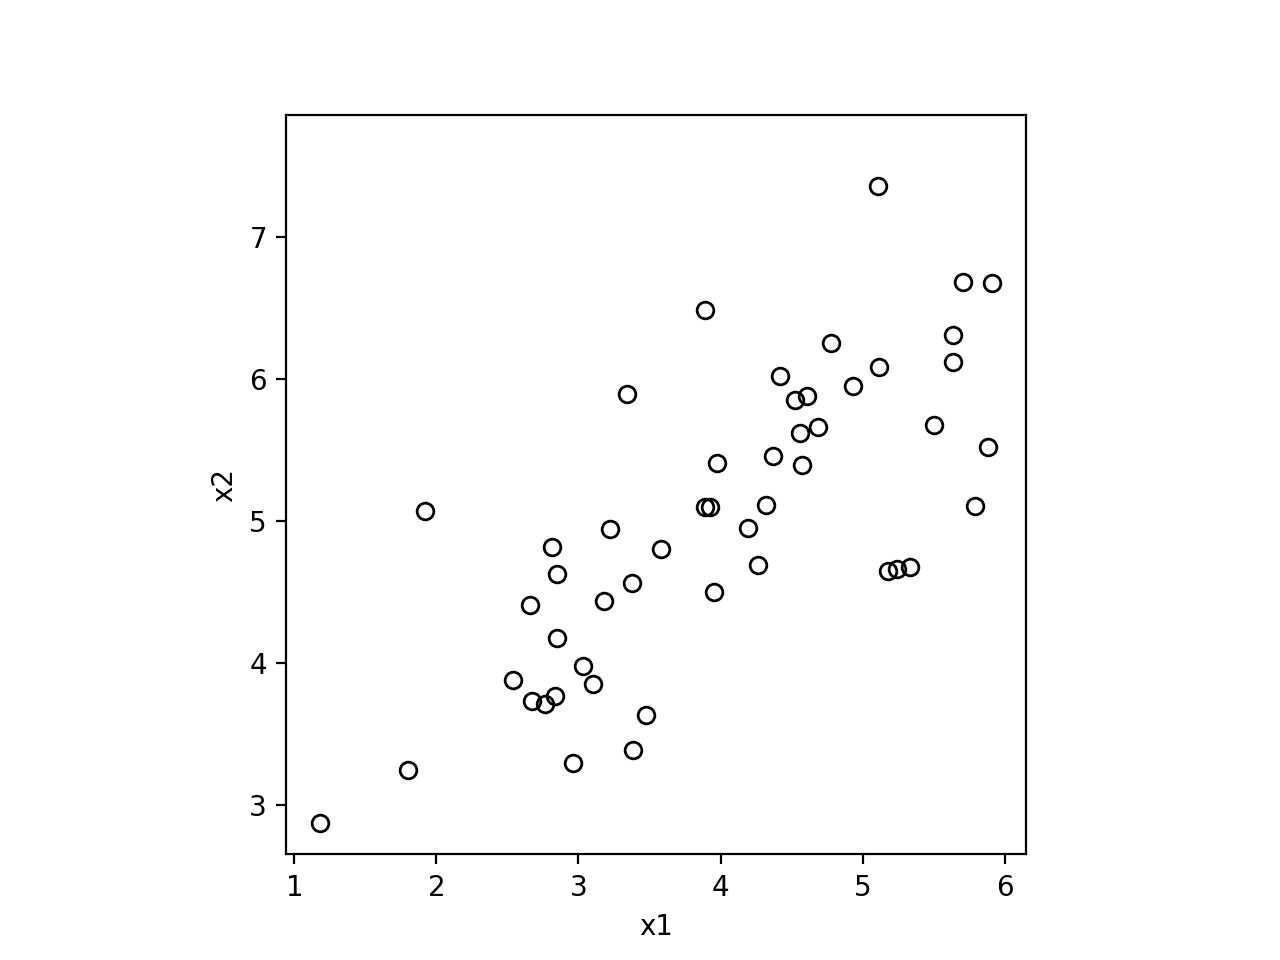
\includegraphics[width=0.5\linewidth]{figs/Chap_12_Figure_0.png}
\end{figure}

主成分分析代码：

\begin{lstlisting}[language=Python]
def PCA(X, dim = -1):
	"""
	X is the input data: (m, n)

	dim is the dimension after reduction
	if dim=-1, then the program select the smallest dim
	such that 99% of variance is retained
	
	return the data after reduction: (m, dim)
	and the data recovered from reduced data: (m, n)
	"""
	Xmean = np.empty((1, X.shape[1]))
	Xstd = np.empty((1, X.shape[1]))
	def normalization(X, k):
		global Xmean, Xstd
		if k == 1:
			Xmean = np.mean(X, axis=0)
			Xstd = np.std(X, axis=0, ddof=1)
			return (X - Xmean) / Xstd
		else:
			return X * Xstd + Xmean

	Xnorm = normalization(X, 1)
	u, s, v = np.linalg.svd(Xnorm.T @ Xnorm)
	if dim == -1:
		dim = 1
		while s[:dim].sum() / s.sum() < 0.99:
			dim += 1
	return Xnorm @ u[:, :dim], normalization(Xnorm @ u[:, :dim] @ u[:, :dim].T, 0)
\end{lstlisting}

得到映射的点：

\begin{figure}[H]
    \centering
    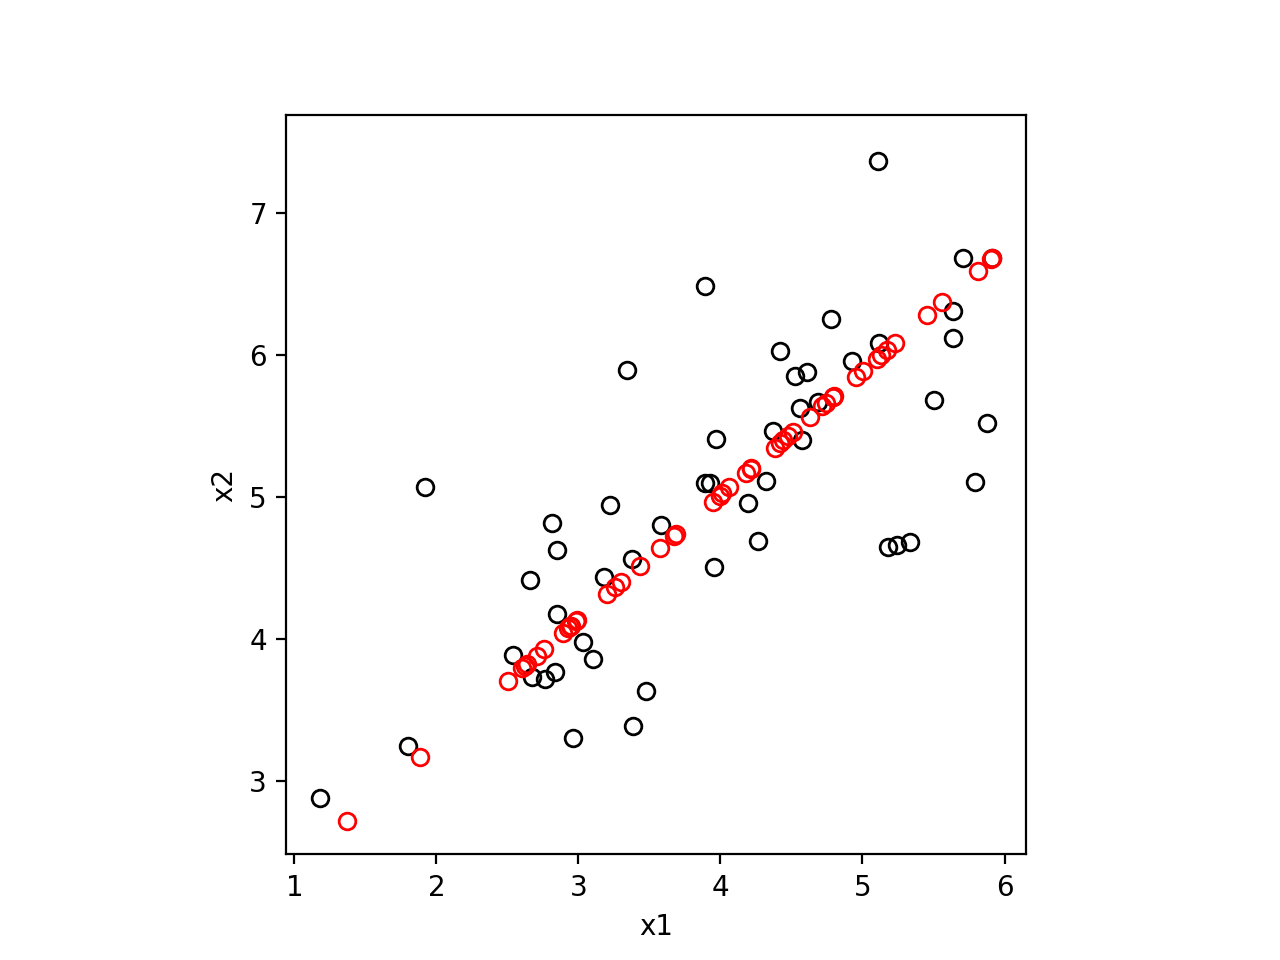
\includegraphics[width=0.5\linewidth]{figs/Chap_12_Figure_1.png}
\end{figure}

\paragraph{人脸特征压缩}

我们给出了 $5000$ 张人脸照片，每张照片含有 $32\times32$ 的灰度像素，形成维度为 $1024$ 的向量作为其特征。前 $100$ 张照片如图所示：

\begin{figure}[H]
    \centering
    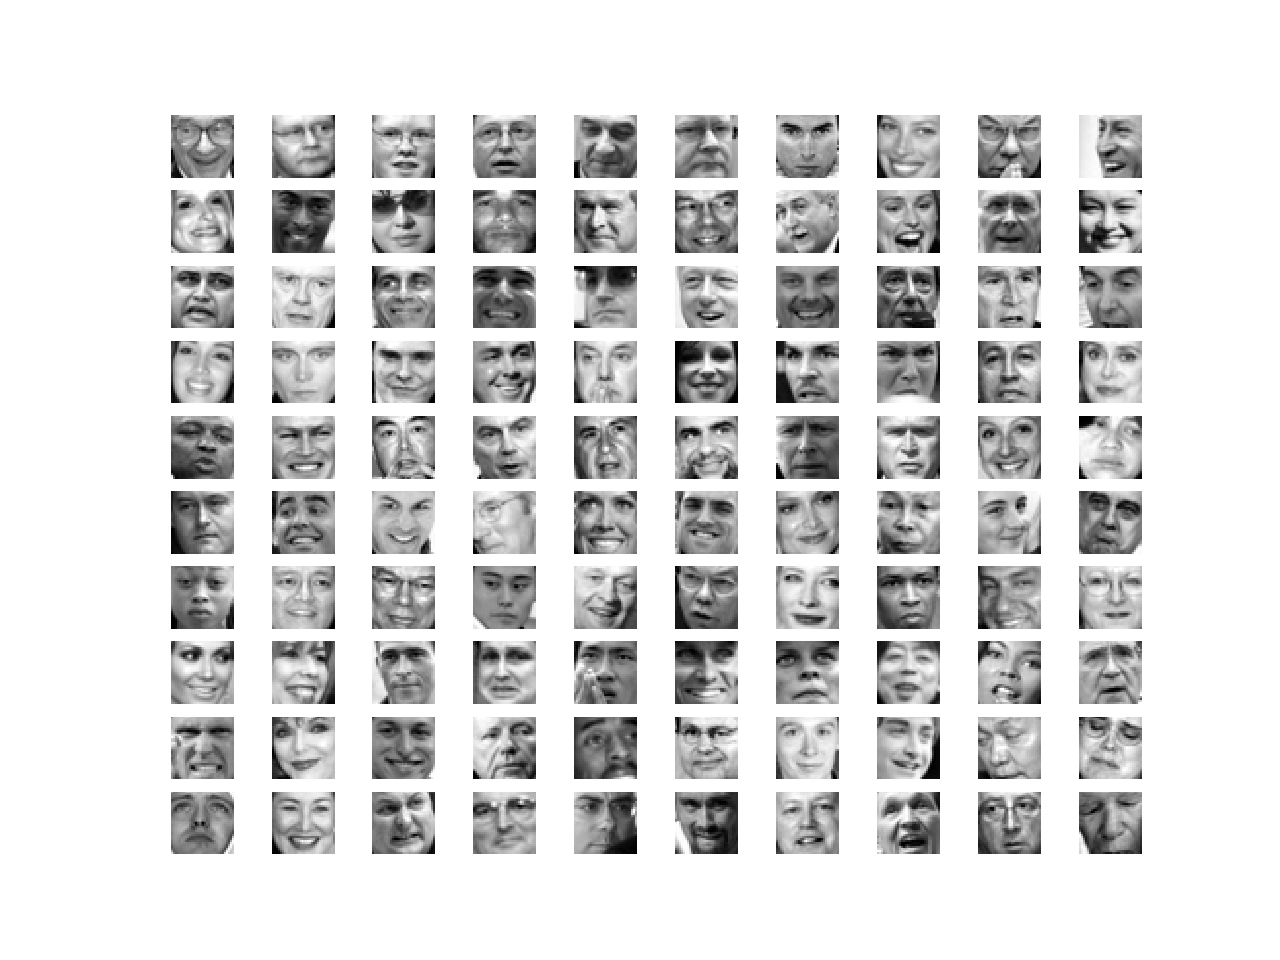
\includegraphics[width=\linewidth]{figs/Chap_12_Figure_2.png}
\end{figure}

现在将其压缩为 $\text{dim}={36,100}$ 维的数据，恢复后结果如下：

\begin{figure}[H]
    \centering
    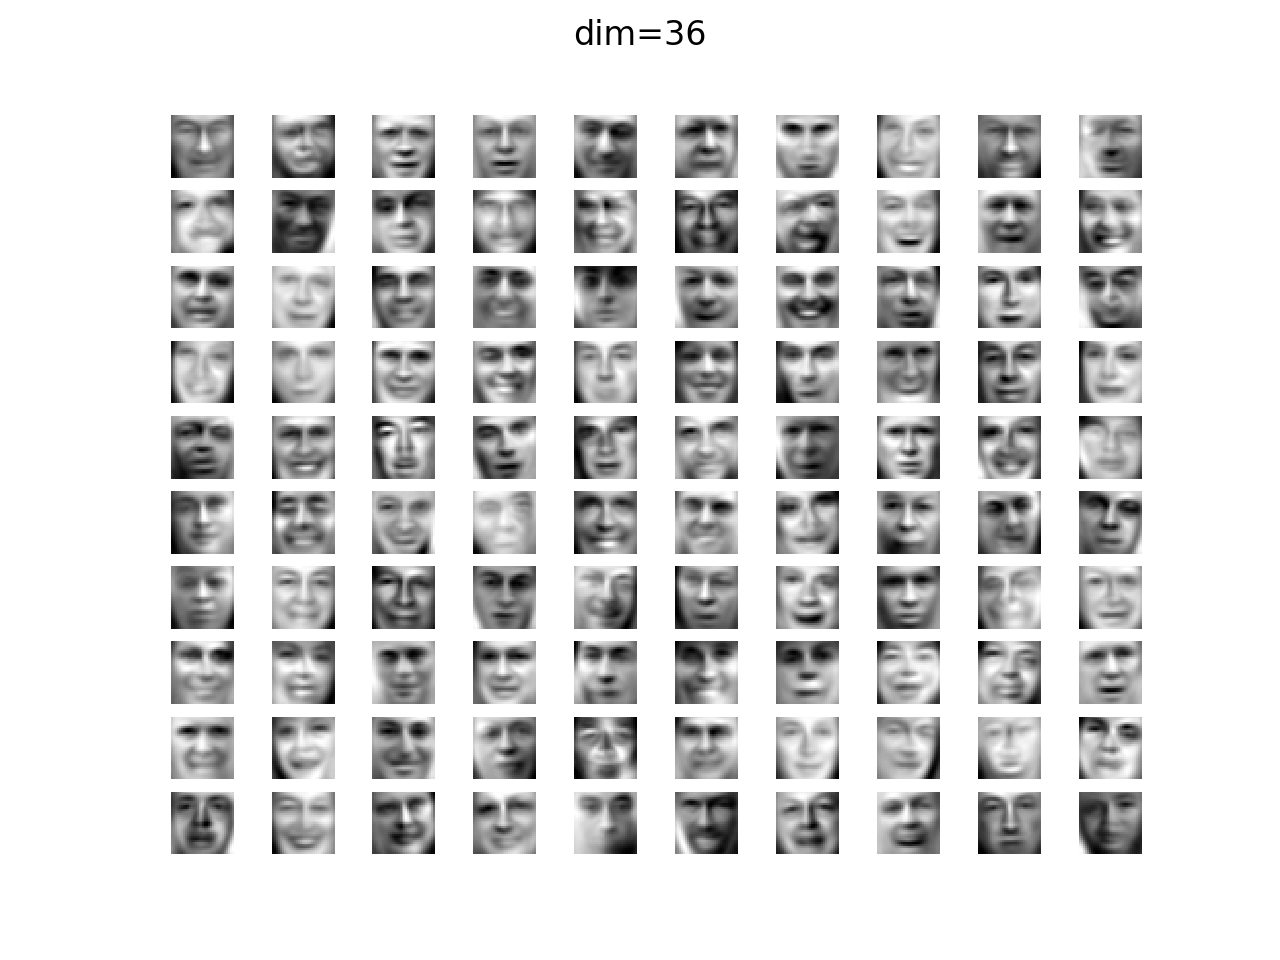
\includegraphics[width=\linewidth]{figs/Chap_12_Figure_dim=36.png}
\end{figure}

\begin{figure}[H]
    \centering
    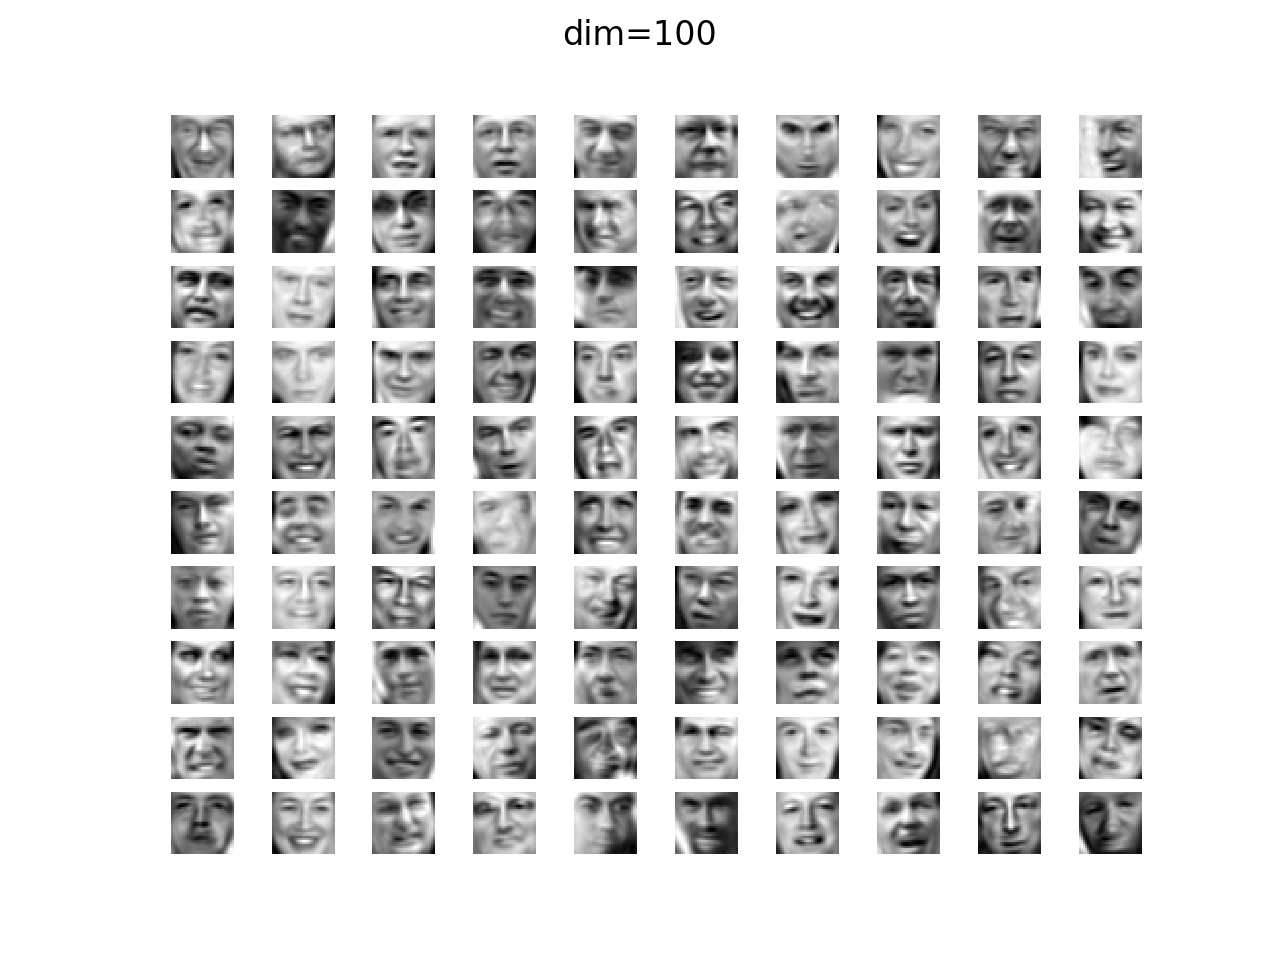
\includegraphics[width=\linewidth]{figs/Chap_12_Figure_dim=100.png}
\end{figure}
